%\newpage
\section{Měření odporů}
Každý odpor se měří čtyřmi měřicími metodami v jednom směru proudu.
Stejný odpor je měřen stejnými čtyřmi měřicími metodami v druhém směru proudu.
Měření v opačném směru se používá pouze pro detekci odporu.
Pokud je odchylka těchto dvou měření příliš velká, není to žádný odpor.

\subsection{Měření odporů s pomocí \(680\Omega\) odporů}
Měření neznámého odporu Rx se provádí dvěma různými způsoby s přesnými odpory \(680\Omega\).
Schéma zapojení těchto měření pomocí zkušebního kolíku 1 (TP1) a zkušebního kolíku 3 (TP3)
je zjednodušeně znázorněno na obr.~\ref{fig:RL1mes} a obrázku~\ref{fig:RL2mes} jako příklad
šesti možných kombinací.

\begin{figure}[H]
\centering
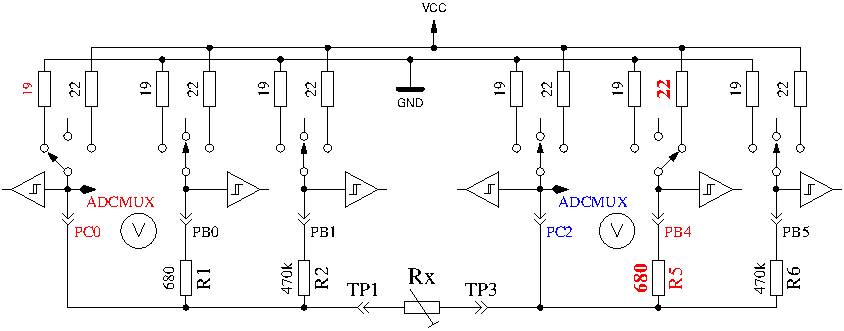
\includegraphics[width=.8\textwidth]{../FIG/ResistormessL1.pdf}
\caption{Měření typu 1 s \(680\Omega\) }
\label{fig:RL1mes}
\end{figure}

\begin{figure}[H]
 \centering
 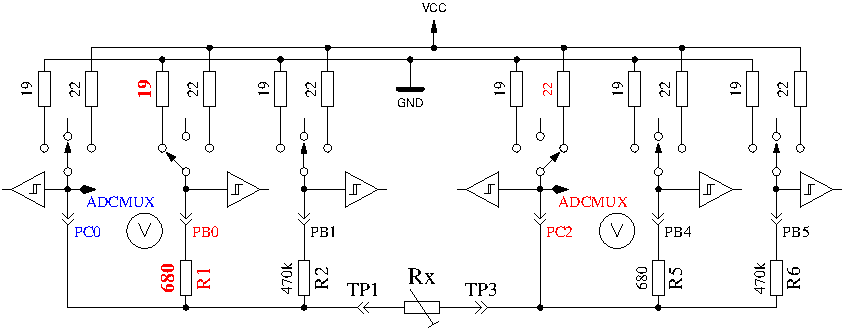
\includegraphics[width=.8\textwidth]{../FIG/ResistormessL2.pdf}
 \caption{Měření typu 2 s \(680\Omega\) }
\label{fig:RL2mes}
\end{figure}

Zkušební pin TP 1 je zobrazen na levé straně a zkušební pin TP 3 na pravé straně.
V obou obvodech je vidět, že je port 3 (TP3) spínán k VCC a na levé straně (TP1)
je připojen na zem GND.
Aktuální směr přes rezistor Rx je vždy stejný.
Hodnoty pro porty přepojené na výstup jsou zobrazeny červeně,
hodnoty vstupů jsou zobrazeny modře, neaktivní porty jsou černé.
V obou měřených metodách by proud měl mít stejnou hodnotu, protože součet odporů mezi
VCC a GND je stejný, pokud jsou vestavěné odpory Atmega stejné.
Vzhledem k tomu, že se pořadí odporů obrací, obvykle nejsou měřené napětí stejné.
Symbol V uvnitř kruhu označuje porty použité pro měření napětí.

V obou konfiguracích je možné, hodnotu odporu Rx vypočítat, ze známých odporů
a měřeného napětí, když poměr odporu Rx a \(680\Omega\) odporů není příliš vysoký.
Teoretická křivka napětí je znázorněna na obr. \ref{fig:RLvtot} kde jsou hodnoty odporu
v logaritmickém měřítku.
\begin{figure}[H]
\centering
\includegraphics[width=.8\textwidth]{../GNU/RLvtotCZ.pdf}
\caption{Napětí typu 1 a typu 2 s měřicím odporem \(680\Omega\) }
\label{fig:RLvtot}
\end{figure}
Gradient pro měření typu 1 je zobrazen na obrázku~\ref{fig:RLvlow} s rozložením pro nižší hodnoty odporu.
Jak můžete vidět, potřebujete lepší  ADC rozlišení, než ty možné \(4,9mV\) na \(5V\) ADC odkazu,
abyste získali správné hodnoty odporu od naměřeného napětí pod \(2\Omega\).
Existují pouze tři úrovně ADC s \(5V\) odkazem mezi \(0\Omega\) a \(2\Omega\).
Přepínání rozsahu s volbou AUTOSCALE\_ADC zde může pomoci.
Stejný rozsah šíření pro měření typu 2 je zobrazen na obrázku~\ref{fig:RLvhigh}.
Bohužel nemůžete použít vyšší rozlišení ADC pro metodu měření typu 2,
protože napětí je příliš vysoké a naše ATmega nemá žádné diferenční ADC vstupy.
Měření s odpory \(680\Omega\)  se stávají až do hodnoty odporu \(20k\Omega\)  (napětí je pod
hodnotou \(169mV\)) použito k určení výsledku měření.
Pro odpory vyšší hodnoty se používají k měření odpory \(470k\Omega\).
Průměrná hodnota obou měření se používá k zobrazení hodnoty odporu, pokud je výsledkem všech měření potvrzeno,
že to není žádná jiná součástka.
Je-li použita funkce AUTOSCALE\_ADC a jedno z naměřených napětí je menší než \(0,98V\) pro obě verze,
pro měření s napětím pod \(0,98V\) se použije závažný průměr s faktorem čtyři.
Druhá hodnota je určena s faktorem jedna.
To způsobí o faktor čtyři lepší rozlišení tohoto měření.
Čtvrtý faktor se používá pouze pro procesory ATmega168 a ATmega328, pro ATmega8 se používá jako
faktor vážení dva, když je napětí nižší než \(0,98V\) protože referenční ADC napětí
je zde \(2,56V\) namísto \(1,1V\).
Pokud má ATmega více než 8 Kb flash paměti, bude měření napětí na odporech tak dlouho zpožděno,
dokud nebude zjištěna žádná změna nebo překročen časový limit.
Tímto opatřením nebudou ani velké kondenzátory omylně rozpoznány jako odpory,
a u velkých cívek bude stejnosměrný odpor správně změřen.

\begin{figure}[H]
  \begin{subfigure}[b]{.5\textwidth}
    \centering
    \includegraphics[width=1.\textwidth]{../GNU/RLvlowCZ.pdf}
    \caption{Měření typu 1}
    \label{fig:RLvlow}
  \end{subfigure}
  ~
  \begin{subfigure}[b]{.5\textwidth}
    \centering
    \includegraphics[width=1.\textwidth]{../GNU/RLvhighCZ.pdf}
    \caption{Měření typu 2}
    \label{fig:RLvhigh}
  \end{subfigure}
  \caption{Výňatek teoretické křivky napětí od \(0\Omega\) do \(10\Omega\)}
\end{figure}


\subsection{Měření odporů s precisními odpory \(470k\Omega\)}
Další obrázky~\ref{fig:RH1mes} a \ref{fig:RH2mes} ukazují stejné měřicí metody pro měření s precisními \(470k\Omega\) odpory.
Protože je \(470k\Omega\) v relaci k odporům portu \(22\Omega\) a \(19\Omega\) velmi velký,
lze odpory portů Atmega  pro výpočet hodnoty odporu Rx zanedbat.
Pro obě metody měření s \(470k\Omega\) odpory se měří jen jedno napětí kvůli tomu že je hodnota proudu
tak nízká, že na vnitřních  odporech portů Atmega nelze měřit žádný rozdíl napětí jak by se očekávalo . Křivka teoretického napětí je znázorněna na obrázku ~\ref{fig:RHv} s hodnotami odporu v logaritmickém měřítku.
Teoretický průběh v tomto diagramu končí u \(100M\Omega\), ale možnost testeru je omezen na \(60M\Omega\),
jinak tester předpokládá, že není připojen žádný odpor.
Jako výsledek se používá průměr obou metod měření.
K tomu jsou použity stejné pravidla, které již platí při měření pomocí odporů \(680\Omega\).
Zjistil jsem, že výsledky měření pro všechny typy ATmega jsou bližší skutečné hodnotě,
pokud je k výsledku měření přidán konstantní rozdíl  \(350\Omega\).
Tento ofset lze nastavit pomocí konstantního RH\_OFFSET (definovat) v souboru config.h.

\begin{figure}[H]
\centering
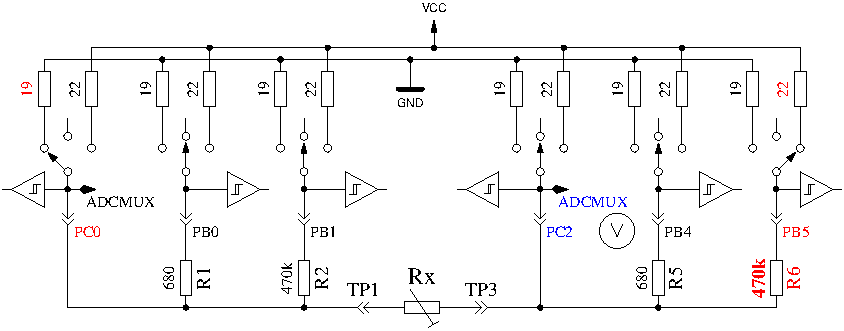
\includegraphics[width=.8\textwidth]{../FIG/ResistormessH1.pdf}
\caption{Měření typu 3 s \(470k\Omega\) }
\label{fig:RH1mes}
\end{figure}

\begin{figure}[H]
 \centering
 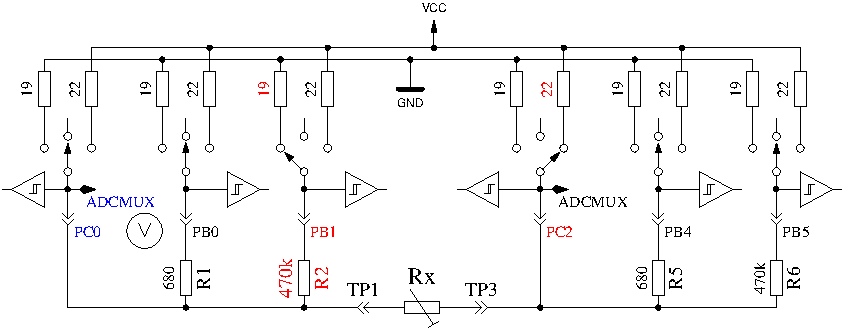
\includegraphics[width=.8\textwidth]{../FIG/ResistormessH2.pdf}
 \caption{Měření typu 4 s \(470k\Omega\) }
\label{fig:RH2mes}
\end{figure}

\begin{figure}[H]
\centering
 \includegraphics[width=.8\textwidth]{../GNU/RHvCZ.pdf}
\caption{Napětí při měření typu 3 a typu 4 s \(470k\Omega\) }
\label{fig:RHv}
\end{figure}

\subsection{Výsledky měření odporů}
Obrázek~\ref{fig:mega8res}  ukazuje relativní chybu měření odporu se třemi různými ATmega8.
Kromě toho jsou výsledky měření některých odporů s původním softwarem Markuse F. zobrazeny jako ,,Mega8orig''.
Výsledky měření stejných odporů se třemi ATmega8A a třemi ATmega8L jsou uvedeny
na obrázcích\ref{fig:mega8Ares} a \ref{fig:mega8Lres}.
Obrázek~\ref{fig:mega168res} ukazuje stejné měření pomocí ATmega168.
,,Mega168'' jsou výsledky bez možnosti AUTOSCALE\_ADC, ,,Mega168as'' s touto možností.
S ATmega168 se zdá být možné získat měření odporu v rozsahu od \(20\Omega\) bis
\(20M\Omega\) s chybou měření menší než  \(\pm1\%\).
Pro měření pod \(100\Omega\)je třeba vzít v úvahu, že každá zkušební šňůra má také nějakou hodnotu odporu.
Je lepší připojit měřěný objekt přímo ke svorkám.
Pokud to není možné, je třeba od výsledku měření odečítat odpor zkratovaných zkušebních šnůr.
Například. Tester zobrazí hodnotu \(30,6\Omega\). Pokud má přesný odpor vytištěnou hodnotu \(30\Omega\)
a zkratované zkušební kabely mají hodnotu  \(0,5\Omega\), pak je skutečná hodnota odporu \(30,1\Omega\).
Pod hodnotou odporu \(10\Omega\), činí krok rozlišení \(0,1\Omega\) již chybu více než \(1\%\)!

\begin{figure}[H]
\centering
 \includegraphics[width=.8\textwidth]{../GNU/Mega8resCZ.pdf}
\caption{Relativní chyba pro měření odporu s ATmega8}
\label{fig:mega8res}
\end{figure}

\begin{figure}[H]
  \begin{subfigure}[b]{.5\textwidth}
    \centering
    \includegraphics[width=1.\textwidth]{../GNU/Mega8AresCZ.pdf}
    \caption{Se třemi ATmega8A}
    \label{fig:mega8Ares}
  \end{subfigure}
  ~
  \begin{subfigure}[b]{.5\textwidth}
    \centering
    \includegraphics[width=1.\textwidth]{../GNU/Mega8LresCZ.pdf}
    \caption{Se třemi ATmega8L}
    \label{fig:mega8Lres}
  \end{subfigure}
\caption{Relativní chyba při měření odporů}
\end{figure}

\begin{figure}[H]
\centering
\includegraphics[width=.8\textwidth]{../GNU/Mega168resCZ.pdf}
\caption{Relativní chyba při měření odporů s ATmega168}
\label{fig:mega168res}
\end{figure}

Diagram \ref{fig:m168res_all} ukazuje chyby měření tří procesorů ATmega168 před kalibrací jako body,
po kterých kalibrace jako přímka.
Tomu odpovídá  měření chyb u tří ATmega168A na obr. \ref{fig:m168ares_all} a tří ATmega328P
zobrazených na obrázku \ref{fig:m168pres_all}.
Chyby měření ATmega328 jsou zobrazeny na obrázcích \ref{fig:m328res_all} a \ref{fig:m328pres_all}.
Po automatické kalibraci zůstává chyba měření v rozsahu odporu s jednou výjimkou (ATmega328P-13, \(22k\Omega\)), 
\(10\Omega~-~20M\Omega\) v rozsahu \(\pm1\%\).
Před kalibrací dosahovaly chyby měření v některých procesorech až \(\pm~3\%\).
Chyba je způsobena přepnutím ADC reference AUTOSCALE\_ADC.
Přímým porovnáním napětí kondenzátoru pod \(1V\), jednou s VCC odkazem a opět s měřením interní referencí , může být chyba kompenzována.
V tomto případě je napětí měřeno stejným kanálem multiplexeru a referenční pásmo je na AREF kolíku
zapnuté.
Přímé měření (Bandgap-reference) přímou volbou vstupu multiplexeru bohužel vede k tomuto ofsetu,
který lze ručně odstranit pomocí volby REF\_R\_KORR nebo automaticky s volbou AUTO\_CAL auto-testu.
V režimu AUTO\_CAL-Modus je REF\_R\_KORR další ofset k automaticky zjištěnému rozdílu napětí.

\begin{figure}[H]
  \begin{subfigure}[b]{.5\textwidth}
    \centering
    \includegraphics[width=1.\textwidth]{../GNU/m168res_allCZ.pdf}
    \caption{Se třemi ATmega168}
    \label{fig:m168res_all}
  \end{subfigure}
  ~
  \begin{subfigure}[b]{.5\textwidth}
    \centering
    \includegraphics[width=1.\textwidth]{../GNU/m168ares_allCZ.pdf}
    \caption{Se třemi ATmega168A}
    \label{fig:m168ares_all}
  \end{subfigure}
\caption{Relativní chyba při měření odporů}
\end{figure}

\begin{figure}[H]
\centering
\includegraphics[width=.8\textwidth]{../GNU/m168pres_allCZ.pdf}
\caption{Relativní chyba při měření odporů se třemi ATmega168P }
\label{fig:m168pres_all}
\end{figure}

\begin{figure}[H]
  \begin{subfigure}[b]{.5\textwidth}
    \centering
    \includegraphics[width=1.\textwidth]{../GNU/m328res_allCZ.pdf}
    \caption{Se třemi ATmega328}
    \label{fig:m328res_all}
  \end{subfigure}
  ~
  \begin{subfigure}[b]{.5\textwidth}
    \centering
    \includegraphics[width=1.\textwidth]{../GNU/m328pres_allCZ.pdf}
    \caption{Se třemi ATmega328P}
    \label{fig:m328pres_all}
  \end{subfigure}
\caption{Relativní chyba při měření odporů}
\end{figure}

